\documentclass{standalone}

\usepackage{tikz}
\usepackage[outline]{contour}

\begin{document}
  %noformat{
  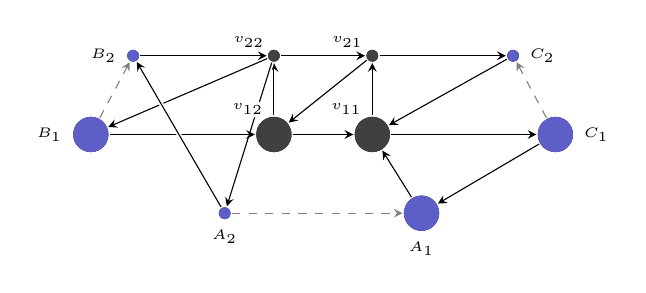
\begin{tikzpicture}
    \contourlength{1.2pt}
    \tikzstyle{v1} = [circle, outer xsep=0.5pt, fill, inner sep=1.5pt]
    \tikzstyle{v2} = [circle, outer xsep=0.5pt, fill, inner sep=3.0pt]
    \tikzstyle{v3} = [circle, outer xsep=0.5pt, fill, inner sep=4.5pt]
    \tikzstyle{unf} = [color=darkgray]
    \tikzstyle{frz} = [color=blue!60!darkgray!70]
    \tikzstyle{e} = [->, >={stealth}, preaction={draw=white, -, ultra thick}]
    \tikzstyle{h} = [dashed, color=gray, ->, >={stealth}]
    \tikzstyle{r} = [->, color=red!70!darkgray!70, >={stealth}]

    \tikzset{font=\tiny}

    \coordinate[v3] (v11) at (2.5,1.0) {};
    \coordinate[v3] (v12) at (1.25,1.0) {};
    \coordinate[v1] (v21) at (2.5,2.0) {};
    \coordinate[v1] (v22) at (1.25,2.0) {};
    \coordinate[v3] (B1) at (-1.075,1.0) {};
    \coordinate[v1] (B2) at (-0.5375,2.0) {};
    \coordinate[v3] (C1) at (4.825,1.0) {};
    \coordinate[v1] (C2) at (4.2875,2.0) {};
    \coordinate[v3] (A1) at (3.125,-0.0) {};
    \coordinate[v1] (A2) at (0.625,-0.0) {};

    \draw[e] (v11) -- (v21);
    \draw[e] (v11) -- (C1);
    \draw[e] (v12) -- (v11);
    \draw[e] (v12) -- (v22);
    \draw[e] (v21) -- (v12);
    \draw[e] (v21) -- (C2);
    \draw[e] (v22) -- (v21);
    \draw[e] (v22) -- (B1);
    \draw[e] (v22) -- (A2);
    \draw[e] (B1) -- (v12);
    \draw[h] (B1) -- (B2);
    \draw[e] (B2) -- (v22);
    \draw[h] (C1) -- (C2);
    \draw[e] (C1) -- (A1);
    \draw[e] (C2) -- (v11);
    \draw[e] (A1) -- (v11);
    \draw[e] (A2) -- (B2);
    \draw[h] (A2) -- (A1);

    \node[v3,label={[label distance=-3pt]95:{\contour{white}{$v_{11}$}}}, unf] (n_v11) at (v11) {};
    \node[v3,label={[label distance=-3pt]95:{\contour{white}{$v_{12}$}}}, unf] (n_v12) at (v12) {};
    \node[v1,label={[label distance=-3pt]95:{\contour{white}{$v_{21}$}}}, unf] (n_v21) at (v21) {};
    \node[v1,label={[label distance=-3pt]95:{\contour{white}{$v_{22}$}}}, unf] (n_v22) at (v22) {};
    \node[v3,label={180:{\contour{white}{$B_{1}$}}}, frz] (n_B1) at (B1) {};
    \node[v1,label={180:{\contour{white}{$B_{2}$}}}, frz] (n_B2) at (B2) {};
    \node[v3,label={0:{\contour{white}{$C_{1}$}}}, frz] (n_C1) at (C1) {};
    \node[v1,label={0:{\contour{white}{$C_{2}$}}}, frz] (n_C2) at (C2) {};
    \node[v3,label={270:{\contour{white}{$A_{1}$}}}, frz] (n_A1) at (A1) {};
    \node[v1,label={270:{\contour{white}{$A_{2}$}}}, frz] (n_A2) at (A2) {};
  \end{tikzpicture}
  %}noformat
\end{document}

